
%(BEGIN_QUESTION)
% Copyright 2013, Tony R. Kuphaldt, released under the Creative Commons Attribution License (v 1.0)
% This means you may do almost anything with this work of mine, so long as you give me proper credit

Connect an ``ice-cube'' relay to a low-voltage DC source as well as 120 volts AC so that a hand-operated switch will control the energization of a 120 VAC load.  All electrical connections must be made using a terminal strip (no twisted wires, crimp splices, wire nuts, spring clips, or ``alligator'' clips permitted), and the 120 VAC portion of the circuit must be fused for overcurrent protection.

This exercise tests your ability to properly interpret the ``pinout'' of an electromechanical relay, properly wire a switch to control a relay's coil, properly wire a load to the contacts of a relay, properly select NO/NC contacts on both the switch and the relay, and use a terminal strip to organize all electrical connections.

$$\includegraphics[width=15.5cm]{i03772x01.eps}$$

\vskip 10pt

The following components and materials will be available to you during the exam: assorted ``ice cube'' {\bf relays} with DC-rated coils and matching {\bf sockets} ; assorted pushbutton {\bf switches} ; {\bf terminal strips} ; lengths of {\bf hook-up wire} ; {\bf battery clips} (holders) ; 120 VAC {\bf power cord} with {\bf fuse assembly} ; 120 VAC {\bf lamp or other suitable load}.

\vskip 10pt

You will be expected to supply your own screwdrivers and multimeter for assembling and testing the circuit at your desk.  The instructor will supply the battery(ies) to power your circuit when you are ready to see if it works.  Until that time, your circuit will remain unpowered.

\vskip 20pt

\noindent
{\bf Load/switch status} (instructor chooses): \hskip 20pt \underbar{\hskip 20pt} On when pressed \hskip 10pt {\it or} \hskip 10pt \underbar{\hskip 20pt} Off when pressed

\vfil

Study reference: the ``Control Relays'' section of {\it Lessons In Industrial Instrumentation}.

\underbar{file i03772}
\eject
%(END_QUESTION)





%(BEGIN_ANSWER)


%(END_ANSWER)





%(BEGIN_NOTES)


%INDEX% Mastery exam performance exercise (circuit), relay energization

%(END_NOTES)


